\documentclass[crop=true,tikz,border=1pt,varwidth=8in]{standalone}

%\makeatletter
%%%%%%%%%%%%%%%%%
\PassOptionsToPackage{force}{filehook}
\usepackage{tikz}
\usetikzlibrary{shapes,arrows}
\usetikzlibrary{positioning}
\tikzstyle{cloud} = [rectangle, draw=black!50, fill=black!20, thick, minimum width=0.6cm,
minimum height = 1cm]
\tikzstyle{line} = [draw, -latex', color=yellow]
\usetikzlibrary{shapes.symbols,shapes.callouts,patterns}
\usetikzlibrary{calc}


\begin{document}
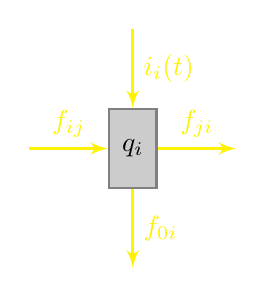
\begin{tikzpicture}[auto]
	\node [cloud] (S) {$q_i$};
	\coordinate[above=of S] (h1);
	\coordinate[right=of S] (h2);
	\coordinate[left=of S] (h3);
	\coordinate[below=of S] (h4);
	%% Flows
	\path [line, very thick] (h1) to node [midway, right] (TextNode) {$i_i(t)$} (S);
	\path [line, very thick] (S) to node [midway, above] (TextNode) {$f_{ji}$} (h2);
	\path [line, very thick] (h3) to node [midway, above] (TextNode) {$f_{ij}$} (S);
	\path [line, very thick] (S) to node [midway, right] (TextNode) {$f_{0i}$} (h4);
\end{tikzpicture}
\end{document}